\subsection{Beam-Induced Heating}
\label{sec:beam-heating-tctp}

As seen in Sec.~\ref{sec:imp-sims-tctp}, the longitudinal impedance of the phase 2 RF design indicates a significant number of beam impedance resonances below 1GHz. Although their contribution in the imaginary component of the beam coupling impedance is not significant enough to be of concern from a stability point of view, the resonances may present a problem from the point of view of beam-induced heating. To fully investigate both the effectiveness of the ferrite in damping the cavity resonances and to identify the locations of the power loss the phase 2 structure is investigated using the frequency domain code HFSS. 

For these simulations we simulate half of the structure (due to the reflective symmetry in the longitudinal plane), using alternatively perfect E-field (enforcing perpendicular electric fields at the boundary) and H-field (enforcing perpendicular magnetic fields at the boundary) boundary conditions at the symmetry plane to indentify and characterise the eigenmodes up to 2GHz (to cover the majority of the beam spectrum). The structure with and without ferrite is simulated to characterise the effect of the ferrite in damping the cavity modes. Simulations are carried out using the following parameters:

\begin{itemize}
\item{Using a 2$^{nd}$ order basis function solver to ensure good resolution of the fields for R/Q and localised loss calculations.}
\item{The ferrite is assumed to be 4A4, materials data is imported from an external data file and interpretted fit is used between data points. An analytical model (see [cite entry] for details).}
\item{We simulate using a single jaw seperation, in this case a half-seperation of 2mm. This is an extremely close jaw seperation, closer in fact than the TCTP collimator would be placed at, but similar to that that the phase 2 collimators would be placed at. This allows some prediction of a worst case scenario for the TCTP and also an analysis of the efficacy of the RF system for the type of operational parameters the phase 2 secondary collimators would be placed at.}
\item{The mesh was auto-generated by the HFSS mesh generator, and run for a convergence criteria of a 0.5\% convergence of the eigenmode frequency between two successive meshes with a 30\% refinement of the mesh between successive solutions.}
\end{itemize}

\begin{figure}
\begin{center}
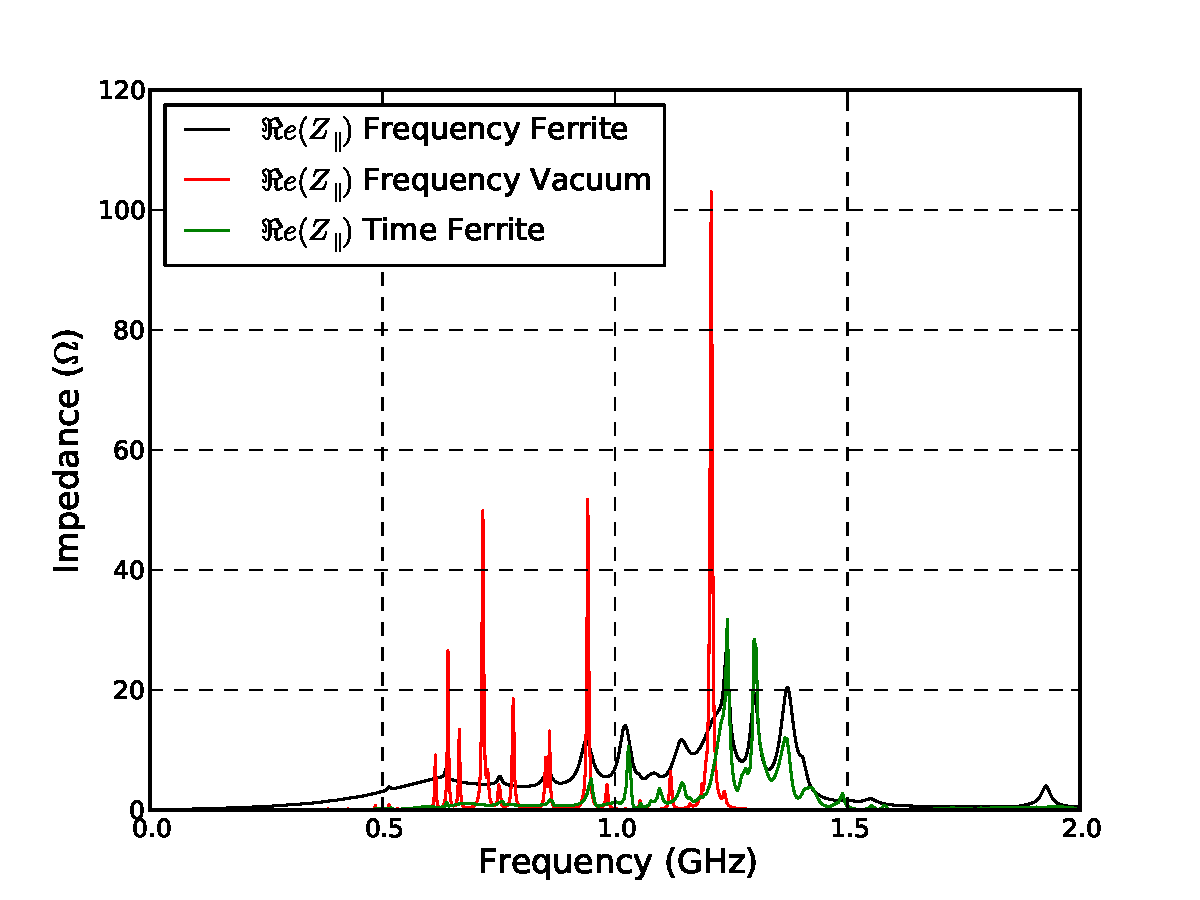
\includegraphics[width=0.7\textwidth]{LHC_Collimation_Upgrades/figures/longitudinal-impedance-tctp-ferr-freq-dom.pdf}
\end{center}
\label{fig:long-imp-tctp-freq}
\caption{The real component of the longitudinal impedance for the TCTP collimator as simulated by both the time and frequency domains for the case with and without ferrite damping tiles. The strong resonances present in the case without ferrite can be seen to be strongly damped when the ferrite tiles are added. However a substantial broadband component occurs in addition due to the broadened resonance peaks.}
\end{figure}

Here we shall evaluate the resonances as a whole, or a few key resonances from a heating point of view. For a complete listing of the eigenmodes please see App.~\ref{app:tctp-eigenmodes} for a complete breakdown of the TCTP eigenmode simulations. To have a comprehensive review of the heating we consider the following heating possibilities

\begin{itemize}
\item{A beam harmonic occuring exactly on the resonant frequency with a certain bunch profile. Here we consider gaussian and cos$^{2}$ bunch profiles. Parameters for a number of different beam operating modes (summarised in Tab.~\ref{tab:lhc-tctp-heating-para}) are considered.}
\item{Taking theoretical spectra for both 50ns and 25ns bunch spacings. In this case we consider the heating for both nominal operational parameters (1ns bunch length), running conditions from 2012 (bunch length between 1.2-1.4ns) and for HL-LHC parameters. These parameters are summarised in Tab.~\ref{tab:lhc-tctp-heating-para}. Different bunch profiles are considered - gaussian and cos$^{2}$ to account for high frequency lobes observed in measured beam spectra.}
\item{Using measured multi-bunch spectra for 50ns bunch spacing measured in the LHC. These measurements are for the beam from injection, through the ramp to squeeze and finally collisions.}
\end{itemize}

\begin{table}
\caption{The LHC operational parameters considered for heating estimates for the TCTP. Operational parameters include the nominal LHC parameters for 25ns bunch spacing, the peak operational intensity for 50ns bunch spacing used in 2012, and the two possible HL-LHC operational schemes, using both 25ns and 50ns bunch spacing. Here the bunch length is assumed to encompass the $4\sigma$ gaussian width.}
\label{tab:lhc-tctp-heating-para}
\begin{center}
\begin{tabular}{c | c | c | c | c }
Operational Mode & $\tau_{b}$ (ns) & $t_{bunch}$ (ns) & $N_{b}$ & $n_{bunches}$ \\ \hline
50ns, 2012 LHC Operation & 1.2 & 50ns & $1.7 \times 10^{11}$ & 1380 \\ \hline
25ns, Nominal LHC Operation & 1.0 & 25ns & $1.15 \times 10^{11}$ & 2808 \\ \hline
HL-LHC 25ns & 1.0 & 25ns & $2.0 \times 10^{11}$ & 2808 \\ \hline
HL-LHC 50ns & 1.0 & 50ns & $3.3 \times 10^{11}$ & 1380 \\ \hline
\end{tabular}
\end{center}
\end{table}

The heating estimates assuming on resonance beam harmonics can be seen in Tab.~\ref{tab:on-res-heating-tctp} for a variety of bunch lengths between 1-1.5ns assuming gaussian and cos$^{2}$ bunch distributions. The same data for the TCTP without the ferrite damping tiles can be seen in Tab.~\ref{tab:on-res-heating-tctp-no-ferr}. A number of things area immediately evident; 	The addition of the ferrite drastically reduces the power loss in the TCTP collimator, by a factor of $\approx$ 3. In addition, the consideration of the higher frequency lobes in the heating estimates for the TCTP is significant, as can be seen in Fig.~\ref{fig:tctp-heating-bunch-length-per-freq}. In this case the usefulness for the ferrites is clear.

\begin{table}
\label{tab:on-res-heating-tctp}
\caption{The power loss of a the TCTP collimator with ferrite for a number of operational modes in the LHC and HL-LHC assuming each cavity mode falls upon a beam harmonic. All losses are in watts using the parameters found in Tab.~\ref{tab:lhc-tctp-heating-para}}
\begin{center}
\begin{tabular}{c | c | c | c | c | c | c | c | c  }
$\tau_{b}$ (ns) & \multicolumn{2}{| c |}{50ns, 2012} & \multicolumn{2}{| c |}{25ns nominal} & \multicolumn{2}{| c |}{50ns, HL-LHC} & \multicolumn{2}{| c }{25ns, HL-LHC} \\ \hline
 & $P_{loss, g}$ & $P_{loss, c}$ & $P_{loss, g}$ & $P_{loss, c}$ & $P_{loss, g}$ & $P_{loss, c}$ & $P_{loss, g}$ & $P_{loss, c}$ \\ \hline
1.0 & 5.6 & 14.2 & 10.6 & 27.0 & 21 & 53.4 & 32.2 & 81.8 \\ \hline
1.1 & 3.8 & 10.2 & 7.2 & 19.6 & 14.4 & 38.8 & 22.0 & 59.0 \\ \hline
1.2 & 2.6 & 7.4 & 5.0 & 14.0 & 10.2 & 27.8 & 15.4 & 42.2 \\ \hline
1.3 & 2.0 & 5.4 & 3.6 & 10.0 & 7.2 & 20.0 & 11.0 & 30.4 \\ \hline
1.4 & 1.4 & 3.8 & 2.6 & 7.4 & 5.2 & 14.6 & 8.0 & 22.2 \\ \hline
1.5 & 1.0 & 2.8 & 2.0 & 5.4 & 3.8 & 10.8 & 5.8 & 16.4 \\ \hline
\end{tabular}
\end{center}
\end{table}

\begin{table}
\label{tab:on-res-heating-tctp-no-ferr}
\caption{The power loss of a TCTP collimator without the ferrite damping tiles for a number of operational modes in the LHC and HL-LHC assuming each cavity mode falls upon a beam harmonic. All losses are in watts using the parameters found in Tab.~\ref{tab:lhc-tctp-heating-para}}
\begin{center}
\begin{tabular}{c | c | c | c | c | c | c | c | c  }
$\tau_{b}$ (ns) & \multicolumn{2}{| c |}{50ns, 2012} & \multicolumn{2}{| c |}{25ns nominal} & \multicolumn{2}{| c |}{50ns, HL-LHC} & \multicolumn{2}{| c }{25ns, HL-LHC} \\ \hline
 & $P_{loss, g}$ & $P_{loss, c}$ & $P_{loss, g}$ & $P_{loss, c}$ & $P_{loss, g}$ & $P_{loss, c}$ & $P_{loss, g}$ & $P_{loss, c}$ \\ \hline
1.0 & 2.8 & 7.1 & 5.3 & 13.5 & 10.5 & 26.7 & 16.1 & 40.9 \\ \hline
1.1 & 1.9 & 5.1 & 3.6 & 9.8 & 7.2 & 19.4 & 11.0 & 29.5 \\ \hline
1.2 & 1.3 & 3.7 & 2.5 & 7.0 & 5.1 & 13.9 & 7.7 & 21.1 \\ \hline
1.3 & 1.0 & 2.7 &1.8 & 5.0 & 3.6 & 10.0 & 5.5 & 15.2 \\ \hline
1.4 & 0.7 & 1.9 & 1.3 & 3.7 &2.6 & 7.3 & 4.0 & 11.1 \\ \hline
1.5 & 0.5 & 1.4 & 1.0 & 2.7 & 1.9 & 5.4 & 2.9 & 8.2 \\ \hline
\end{tabular}
\end{center}
\end{table}

\begin{figure}
\label{fig:tctp-heating-bunch-length-per-freq}
\caption{The beam-induced heating of the TCTP with ferrite damping tiles for a number of different bunch lengths assuming both a gaussian and cos$^{2}$ distributions.}
\end{figure}

Considering the heating taking beam harmonics seperated the inverse of the bunch seperation (40$MHz$ for $t_{bunch} = 25ns$ and 20$MHz$ for $t_{bunch} = 50ns$) we acquire the results presented in Tab.~\ref{tab:heating-beam-harm-tctp-ferr} and Tab.~\ref{tab:heating-beam-harm-tctp-no-ferr} respectively, again for a variety of LHC operational parameters and assuming either a gaussian or a cos$^{2}$ longitudinal bunch profile. In this case it can be seen that the power loss for the ferrite case is larger than that experienced by the case without ferrite. This can be understood due to the fixed frequencies of the beam harmonics - if a high-Q resonance does not occur at or near a beam harmonic then the beam does not couple to the resonance. Due to the broad resonance peaks of the ferrite damped TCTP design the beam may couple to the resonance even if the resonance frequency of the cavity mode does not match the beam harmonic precisely due to the low-Q of the resonance.

\begin{table}
\label{tab:heating-beam-harm-tctp-ferr}
\caption{The power loss of a TCTP collimator with ferrite for a number of operational modes in the LHC and HL-LHC assuming beam harmonics spaced at the reciprocal of the bunch spacing. All losses are in watts using the parameters found in Tab.~\ref{tab:lhc-tctp-heating-para}}
\begin{center}
\begin{tabular}{c | c | c | c | c | c | c | c | c  }
$\tau_{b}$ (ns) & \multicolumn{2}{| c |}{50ns, 2012} & \multicolumn{2}{| c |}{25ns nominal} & \multicolumn{2}{| c |}{50ns, HL-LHC} & \multicolumn{2}{| c }{25ns, HL-LHC} \\ \hline
 & $P_{loss, g}$ & $P_{loss, c}$ & $P_{loss, g}$ & $P_{loss, c}$ & $P_{loss, g}$ & $P_{loss, c}$ & $P_{loss, g}$ & $P_{loss, c}$ \\ \hline
1.0 & 19.0 & 36.2 & 18.2 & 35.0 & 71.6 & 136.8 & 54.8 & 104.6 \\ \hline
1.1 & 14.8 & 29.2 & 14.2 & 28.0 & 56.2 & 110.0 & 42.8 & 85.0 \\ \hline
1.2 & 11.8 & 23.6 & 11.2 & 22.6 & 44.8 & 89 & 34.0 & 68.6 \\ \hline
1.3 & 9.6 & 19.2 & 9.0 & 18.4 & 36.2 & 72.6 & 27.4 & 55.6 \\ \hline
1.4 & 7.8 & 16.0 & 7.4 & 15.2 & 29.4 & 60.0 & 22.2 & 45.8 \\ \hline
1.5 & 6.4 & 13.2 & 6.0 & 12.6 & 24.2 & 50.0 & 18.4 & 38.0 \\ \hline
\end{tabular}
\end{center}
\end{table}

\begin{table}
\label{tab:heating-beam-harm-tctp-no-ferr}
\caption{The power loss of a TCTP collimator without ferrite for a number of operational modes in the LHC and HL-LHC assuming beam harmonics spaced at the reciprocal of the bunch spacing. All losses are in watts using the parameters found in Tab.~\ref{tab:lhc-tctp-heating-para}}
\begin{center}
\begin{tabular}{c | c | c | c | c | c | c | c | c  }
$\tau_{b}$ (ns) & \multicolumn{2}{| c |}{50ns, 2012} & \multicolumn{2}{| c |}{25ns nominal} & \multicolumn{2}{| c |}{50ns, HL-LHC} & \multicolumn{2}{| c }{25ns, HL-LHC} \\ \hline
 & $P_{loss, g}$ & $P_{loss, c}$ & $P_{loss, g}$ & $P_{loss, c}$ & $P_{loss, g}$ & $P_{loss, c}$ & $P_{loss, g}$ & $P_{loss, c}$ \\ \hline
1.0 & 2.8 & 7.1 & 5.3 & 13.5 & 12.1 & 25.0 & 16.1 & 40.9 \\ \hline
1.1 & 1.9 & 5.1 & 3.6 & 9.8 & 7.2 & 19.4 & 11.0 & 29.5 \\ \hline
1.2 & 1.3 & 3.7 & 2.5 & 7.0 & 5.1 & 13.9 & 7.7 & 21.1 \\ \hline
1.3 & 1.0 & 2.7 &1.8 & 5.0 & 3.6 & 10.0 & 5.5 & 15.2 \\ \hline
1.4 & 0.7 & 1.9 & 1.3 & 3.7 &2.6 & 7.3 & 4.0 & 11.1 \\ \hline
1.5 & 0.5 & 1.4 & 1.0 & 2.7 & 1.9 & 5.4 & 2.9 & 8.2 \\ 
\end{tabular}
\end{center}
\end{table}



\subsubsection{Location of Power Deposition}

\begin{figure}
\subfigure[]{

\label{fig:tctp-ferrite}
}
\subfigure[]{

\label{fig:tctp-long-rf-finger}
}

\label{fig:tctp-heat-loc}
\caption{The different thermally sensitive components of the TCTP collimator. \ref{fig:tctp-ferrite} shows the ferrite tiles, and \ref{fig:tctp-long-rf-finger} the longitudinal RF fingers.}
\end{figure}

Due to the poor cooling available in vacuum (cooled by radiative heating only. Although surrounded by a housing/in contact with surrounded components, the thermal contact between different components within the collimator is poor) it is important to know of the proportion of beam-induced power loss that is lost in thermally sensitive areas. These are areas where large increases in temperature can either lead to direct physical damage (as is the case with RF fingers) or may lead to a worsening physical condition of the collimator (if the ferrite tiles go above their Curie temperature). The components are highlighted in Fig.~\ref{fig:tctp-heat-loc}

The losses on or in different surfaces and volumes is calculated using the loss calculations within HFSS, and then normalised to the total losses in the TCTP structure for each mode. The produces a variety of losses depending on the field pattern of the mode. These are collated in App.~\ref{app:tctp-eigenmodes}. To provide a conservative estimate of the power load we take the highest proportions of power loss of all the modes and assume this is the case for all modes. The percentages for the total device, the ferrite tiles and the longitudinal RF fingers are shown in Tab.~\ref{tab:tctp-heating-loc}. 

\begin{table}
\label{tab:tctp-heating-loc}
\caption{The percentage of power loss lost in thermally sensitive components in the TCTP.}
\begin{center}
\begin{tabular}{c | c}
Component & Percentage of Power Loss \\ \hline
Whole Device & 100 \\ \hline
Ferrite Tiles & 5 \\ \hline
Longitudinal RF Fingers & 4 \\
\end{tabular}
\end{center}
\end{table}

The thermal behaviour as a result of this power load can be analysed using design software such as ANSYS[cite]. The results of these thermal simulations can be seen in [cite F. Carra/M. Garlasche colwg meeting], a summary of which is given in Fig.~\ref{fig:tctp-ferrite-temp-rise}.

\begin{figure}

\label{fig:tctp-ferrite-temp-rise}
\caption{The temperature increase of the ferrite damping tiles in the TCTP collimator under a number of beam operating conditions. Plot taken from [cite Carra and Garlasche]}
\end{figure}